\subsection{Prototypage du premier jeu}


\subsubsection{Le concept}


\begin{wrapfigure}[15]{l}{5cm}
    \vspace{-15pt}
    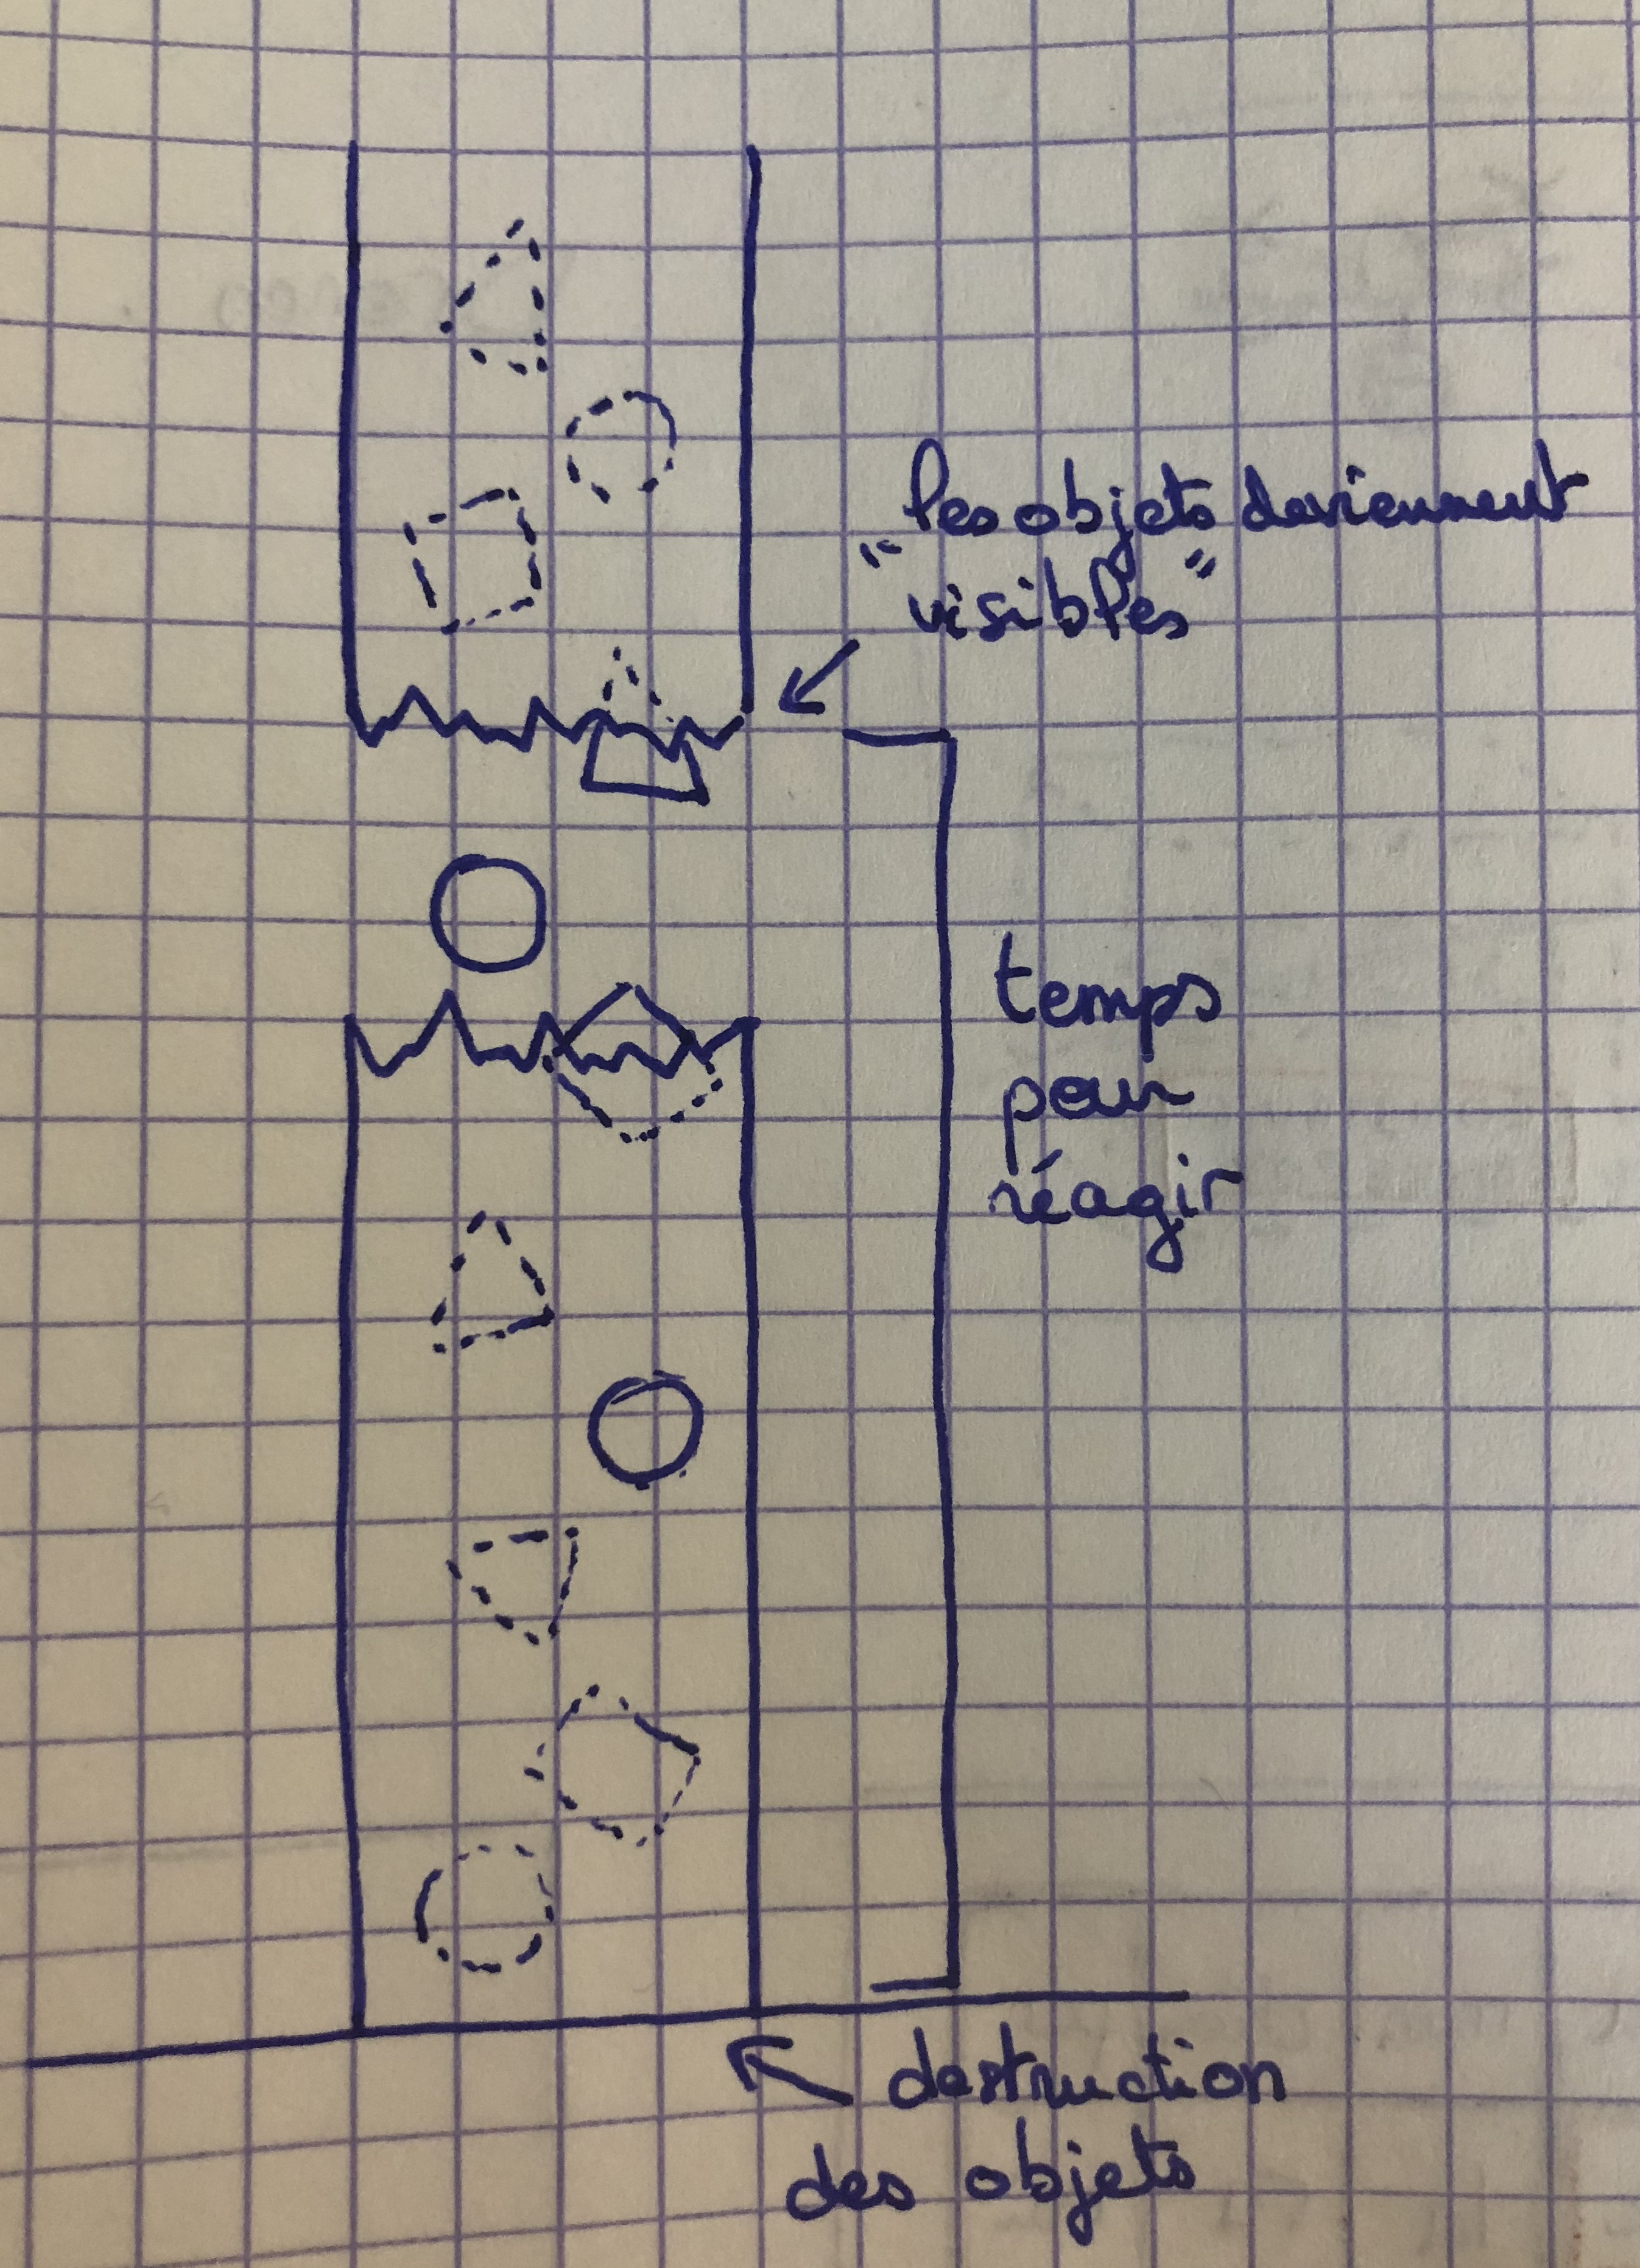
\includegraphics[width=5cm]{temps-reaction.jpg}
    \captionsetup{labelformat=simpleNumber}
    \caption{Temps de réaction}
\end{wrapfigure}

\paragraph{}Nous avons choisi le mini jeu du tuyau comme premier jeu car l'idée était plutôt simple. Il y a un tuyau au milieu de l'écran qui est brisé en son centre. Le
joueur voit des objets tomber par le trou causé par la brisure. Il doit identifier un objet cible parmi tous les autres pour l'enlever du tuyau. Pour éviter de jouer sur ses réflexes,
il faut qu'il puisse interagir avec les objets un peu de temps après qu'ils ne soient plus visibles. Pour cela, le joueur doit pouvoir interagir avec les objets qu'à partir du moment
où il peut les voir, et jusqu'à ce qu'ils soient détruits en atteignant le bas de l'écran.\\ \\

\paragraph{}A chaque fois que le joueur enlève un objet cible, ses points de score augmentent, s'il en loupe ou s'il essaie d'enlever le mauvais objet, ses points de score baissent.
Nous n'étions pas encore sûrs des conditions de victoire :
\begin{itemize}
\item Est-ce que le joueur doit atteindre un certain score avant la fin du temps ?
\item Est-ce que le joueur doit faire le meilleur score en un laps de temps imparti ?
\item Est-ce que le joueur a droit à un nombre d'erreurs maximum ?
\end{itemize}


\paragraph{}Il était également important de définir quels étaient les paramètres à régler. Nous avons pu dégager une première liste de paramètres au préalable, certains
quantifiables, d'autres non.

Parmi les quantifiables :
\begin{itemize}
    \item Vitesse d'apparition/disparition des éléments
    \item Nombre de cibles total ou pourcentage de chance d'apparition de la cible durant la partie
    \item Nombre de distracteurs total ou pourcentage de chance d'apparition du distracteur durant la partie
    \item Emplacement des éléments par rapport au centre
    \item Nombre de cible a trouver pour finir la partie
    \item Temps alloué à la partie
    \item Nombre de distracteurs différents\\
\end{itemize}
Parmi les inquantifiables :
\begin{itemize}
    \item Le design de la cible
    \item Le design des distracteurs
    \item La ressemblance entre la cible et les distracteurs
\end{itemize}

\paragraph{}Pour les touches nous avons choisi pour commencer de garder les mêmes touches que pour la tâche de CPT. Pour enlever les objets, il faudrait alors utiliser la barre espace.
S'il y a plusieurs objets à enlever, cela choisira le premier apparut, donc le plus bas.

\subsubsection{Création de la première scène}

\paragraph{}Pour notre prototype, nous avons commencé par réaliser une première scène plutôt simple. Quelques cylindres représentent le tuyau. Le design n'étant pas très important
dans un premier temps, nous avons fait quelque chose de simple ressemblant un peu à Mario. Un bouton "Start" lance le jeu, remplacé par un bouton "Stop" si l'on veut l'arrêter. Sinon,
la partie continue jusqu'à ce qu'un certain nombre de cibles soit apparues. \\

\begin{figure}[H]
    \begin{center}
    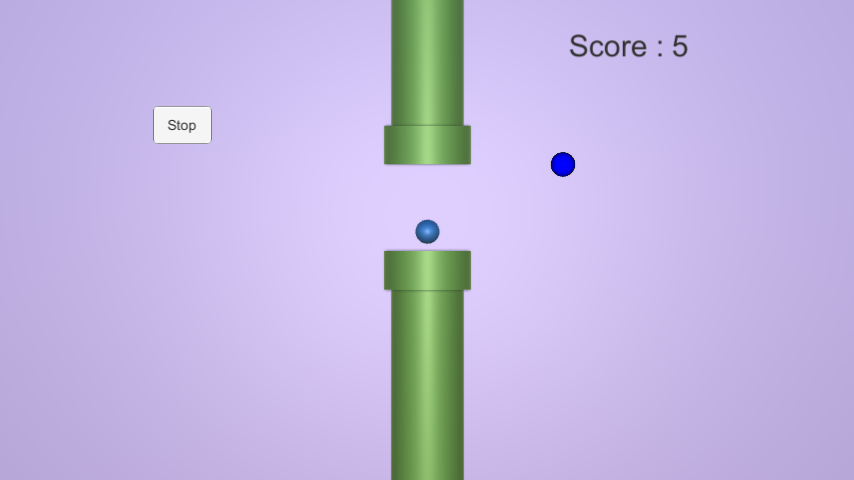
\includegraphics[width=10cm]{proto-pipe1.png}
    \end{center}
    \caption{1\up{er} prototype}
\label{ProtoPipe1}
\end{figure}

\begin{wrapfigure}[9]{l}{3cm}
    \vspace{-10pt}
    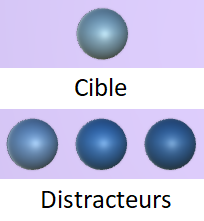
\includegraphics[width=3cm]{proto-pipe-elements.png}
    \captionsetup{labelformat=simpleNumber}
    \caption{Objets}
\end{wrapfigure}

\paragraph{}Les objets dont le joueur doit faire attention sont des boules bleues, plus ou moins claires. La boule la plus claire est la cible, les autres sont les distracteurs. Le
joueur doit être attentif pour enlever la bonne boule. Lorsqu'il en enlève une, celle-ci se déplace jusqu'au point de score pour montrer qu'il a réussi, et le score s'incrémente.
S'il réussit à enlever une cible, il gagne 15 points. S'il en rate une ou s'il essaie d'en enlever une alors qu'il n'y en a pas, il perd 5 points.

\newpage

\paragraph{}Lors d'une partie, nous mesurons la performance d'une personne. Nous en parlerons plus en détail dans la partie \ref{Donnees}. Selon la performance du joueur, nous pouvons
augmenter ou diminuer la difficulté de plusieurs manières.

\paragraph{}D'abord, nous avons cherché à refermer le tube pour que les objets soient visibles pendant moins longtemps. La partie basse du tube peut monter jusqu'à un certain point, les objets
devant rester visibles. Le joueur doit donc être plus attentif.

\paragraph{}Puis, comme le jeu était toujours assez facile, nous avons fait bouger les tubes. Cela n'est pas très clair sur la figure \ref{ProtoPipeDifficultes} mais lorsque le joueur est
performant, le tube se met à trembler tout en pivotant de quelques crans sur la droite ou la gauche. Nous avons mis un angle limite pour éviter une rotation complète du tube.

\paragraph{}Enfin, le jeu étant encore trop facile, nous avons rajouté la possibilité d'ajouter des tuyaux. Il est possible d'en rajouter jusqu'à 5 (ce qu'il est possible d'afficher à l'écran). Le
nombre de tuyaux reste fixe durant une partie, le joueur ne pouvant en rajouter ou en enlever qu'entre deux parties.

\paragraph{}Durant une partie, tous ces paramètres de difficultés peuvent être actifs en même temps. Néanmoins, ceux-ci s'activent selon la performance du joueur : si celui-ci n'est pas très
performant, la difficulté ne bougera pas trop, voire baissera pour s'adapter à son niveau. \\ \\

\begin{figure}[H]
    \begin{center}
    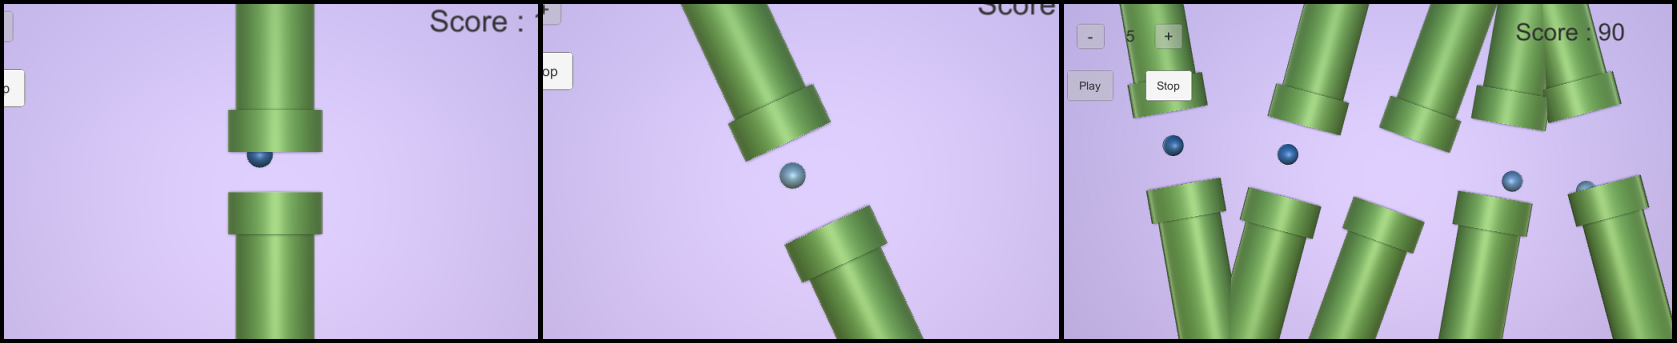
\includegraphics[width=13cm]{proto-pipe-difficultes-evolution.png}
    \end{center}
    \caption{Evolution de la difficulté}
\label{ProtoPipeDifficultes}
\end{figure}

\newpage
\subsubsection{Amélioration du design et du gameplay}

\paragraph{}Après que le prototype soit fonctionnel et validé par les chercheurs, nous avons voulu le rendre un peu plus esthétique. Nous en avons aussi profité pour améliorer le
gameplay et rajouter du contenu. \\


\begin{wrapfigure}[13]{l}{6cm}
    \vspace{-10pt}
    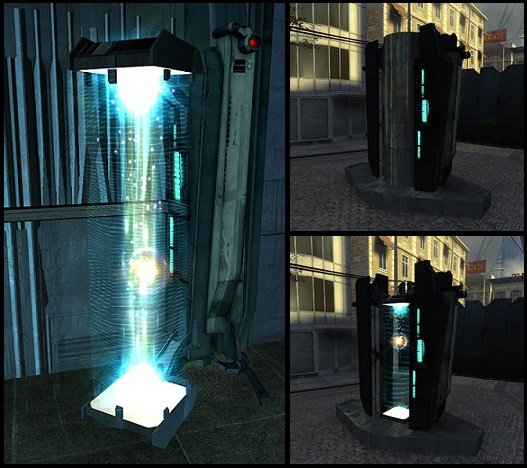
\includegraphics[width=6cm]{hl2-power-generator.jpg}
    \captionsetup{labelformat=simpleNumber}
    \caption{Décor}
\end{wrapfigure}

\paragraph{Contexte}Notre thème est la \gls{SF}. Nous avons donc cherché des inspirations dans des jeux avec cette thématique. L'un d'eux nous est venu assez rapidement à l'esprit.
Il y a dans Half Life 2 des générateurs d'énergie qui ressemble à des tubes dans laquelle une sphère d'énergie flotte. Ces générateurs sont d'abord fermés par une sorte de bouclier
qu'il faut ouvrir pour pouvoir récupérer la sphère d'énergie. Nous avons voulu nous baser sur ce principe pour notre gameplay.

\paragraph{}Nos tubes de Mario sont donc devenus des tubes électromagnétiques, protégés par des boucliers qui peuvent s'ouvrirent en se séparant en deux au milieu. Des sphères
d'énergie descendant le long du tube remplacent les boules bleues et sont maintenant les nouveaux distracteurs et cible.

\begin{figure}[H]
    \begin{center}
    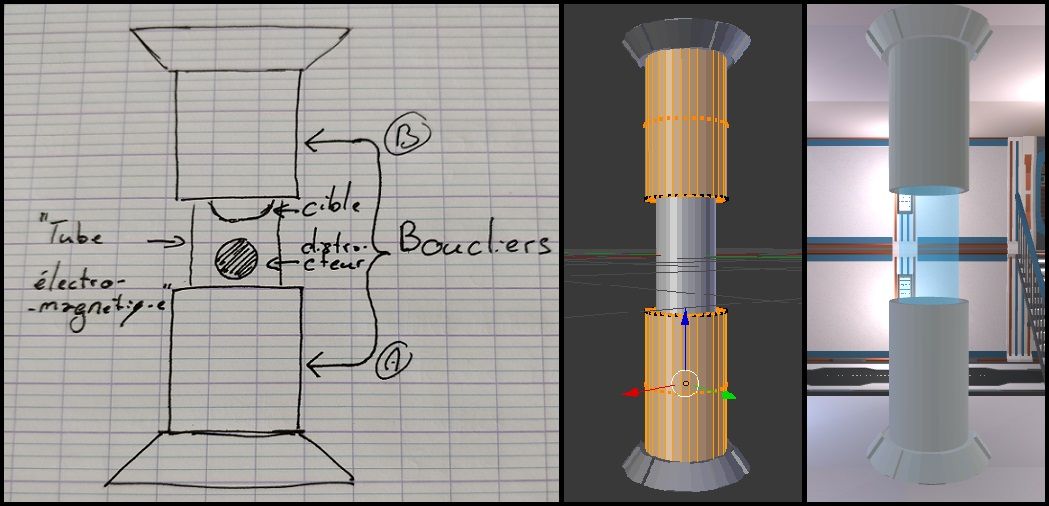
\includegraphics[width=9cm]{PDC-tube-evolution.jpg}
    \end{center}
    \caption{Création des tubes}
\label{TubeEvolution}
\end{figure}

\begin{wrapfigure}[5]{r}{5cm}
    \vspace{-25pt}
    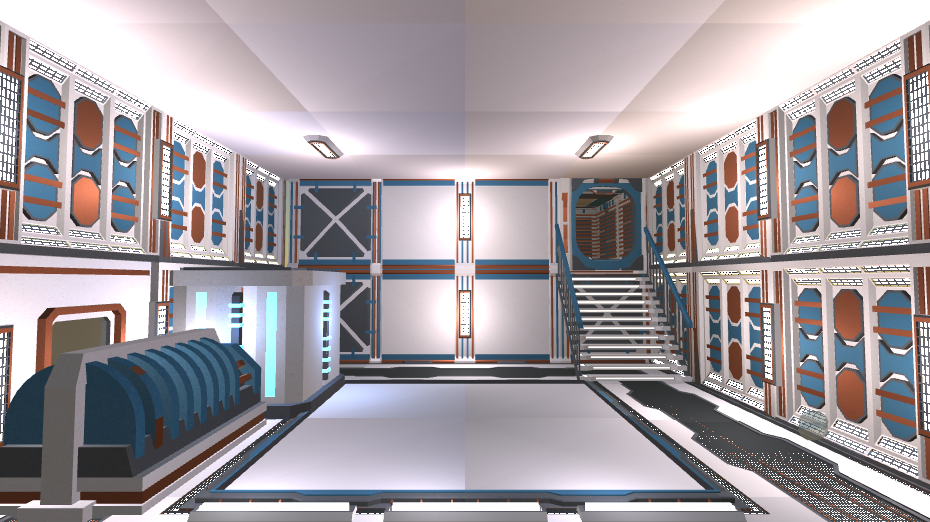
\includegraphics[width=5cm]{PDC-decor.png}
    \captionsetup{labelformat=simpleNumber}
    \caption{Décor}
\end{wrapfigure}

\paragraph{}En parallèle, nous avons construit une scène Unity avec un package de \gls{SF} pour ambiancer le mini jeu. Cette scène représente l'intérieur d'une base scientifique avec
des couleurs plutôt blanches, bleues et oranges.

\newpage

\paragraph{Gameplay}Pour pouvoir intégrer le tube dans la scène, nous avons pensé à le multiplier et le placer sur un barillier qui pourrait tourner. Chaque tube aurait un niveau
d'énergie. Le but du joueur est d'enlever des sphère d'énergie instable (les cibles) pour ne pas que le niveau d'énergie stable d'un des tubes arrive à 0. Si c'est le cas, c'est le
game over. Le joueur peut utiliser les touches droite et gauche du clavier pour faire tourner le barillier et faire face à un autre tube. Il ne peut enlever une sphère instable d'un
tube que lorsque celui-ci lui fait face. Si le joueur est performant, la difficulté peut augmenter de plusieurs manières :
\begin{itemize}
    \item Un nouveau tube s'ouvre
    \item Un des tubes ouverts referme légèrement son bouclier
    \item La couleur des distracteurs se rapproche de celle de la cible
\end{itemize}

\begin{figure}[H]
    \begin{center}
    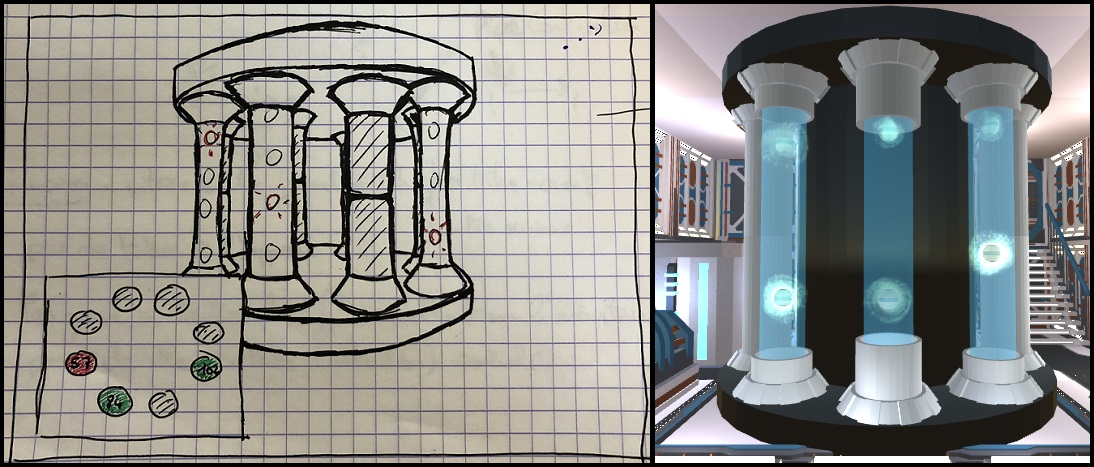
\includegraphics[width=13cm]{PDC-barillier-evolution.jpg}
    \end{center}
    \caption{Barillier de tubes}
\label{BarillierTube}
\end{figure}

\begin{wrapfigure}[5]{l}{4cm}
    \vspace{-25pt}
    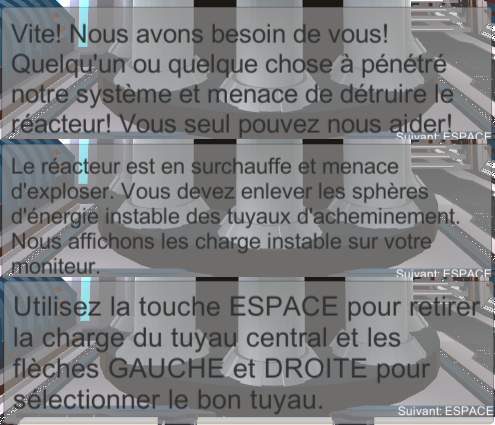
\includegraphics[width=4cm]{PDC-narration.png}
    \captionsetup{labelformat=simpleNumber}
    \caption{Narration}
\end{wrapfigure}

\paragraph{}Les instructions destinées au joueur sont expliquées au début de la première partie d'une session de jeu par la narration. Celle-ci explique le contexte dans lequel se
trouve le mini-jeu, que doit faire le joueur et quelles sont les contrôles à utiliser. \\ \\ \\

\paragraph{Ouverture des tubes}Sur le barillier, seulement 3 tubes accolés maximum sont ouverts à la fois pour des raisons de visibilité des tubes par le joueur. Comme les tubes
s'ouvrent un par un au fur et à mesure de la partie, il fallait un algorithme qui puisse sélectionner le bon tube à ouvrir. L'image \ref{OpenTube} montre les possibilités de tube à
ouvrir que l'algorithme doit pouvoir trouver. Lorsque ces possibilités sont trouvées, on choisit un tube aléatoirement parmi cette liste. Cet algorithme doit pouvoir être assez
générique pour être fonctionnel peu importe le nombre de tubes à ouvrir et peu importe le nombre de tubes sur le barillier.

\begin{figure}[H]
    \begin{center}
    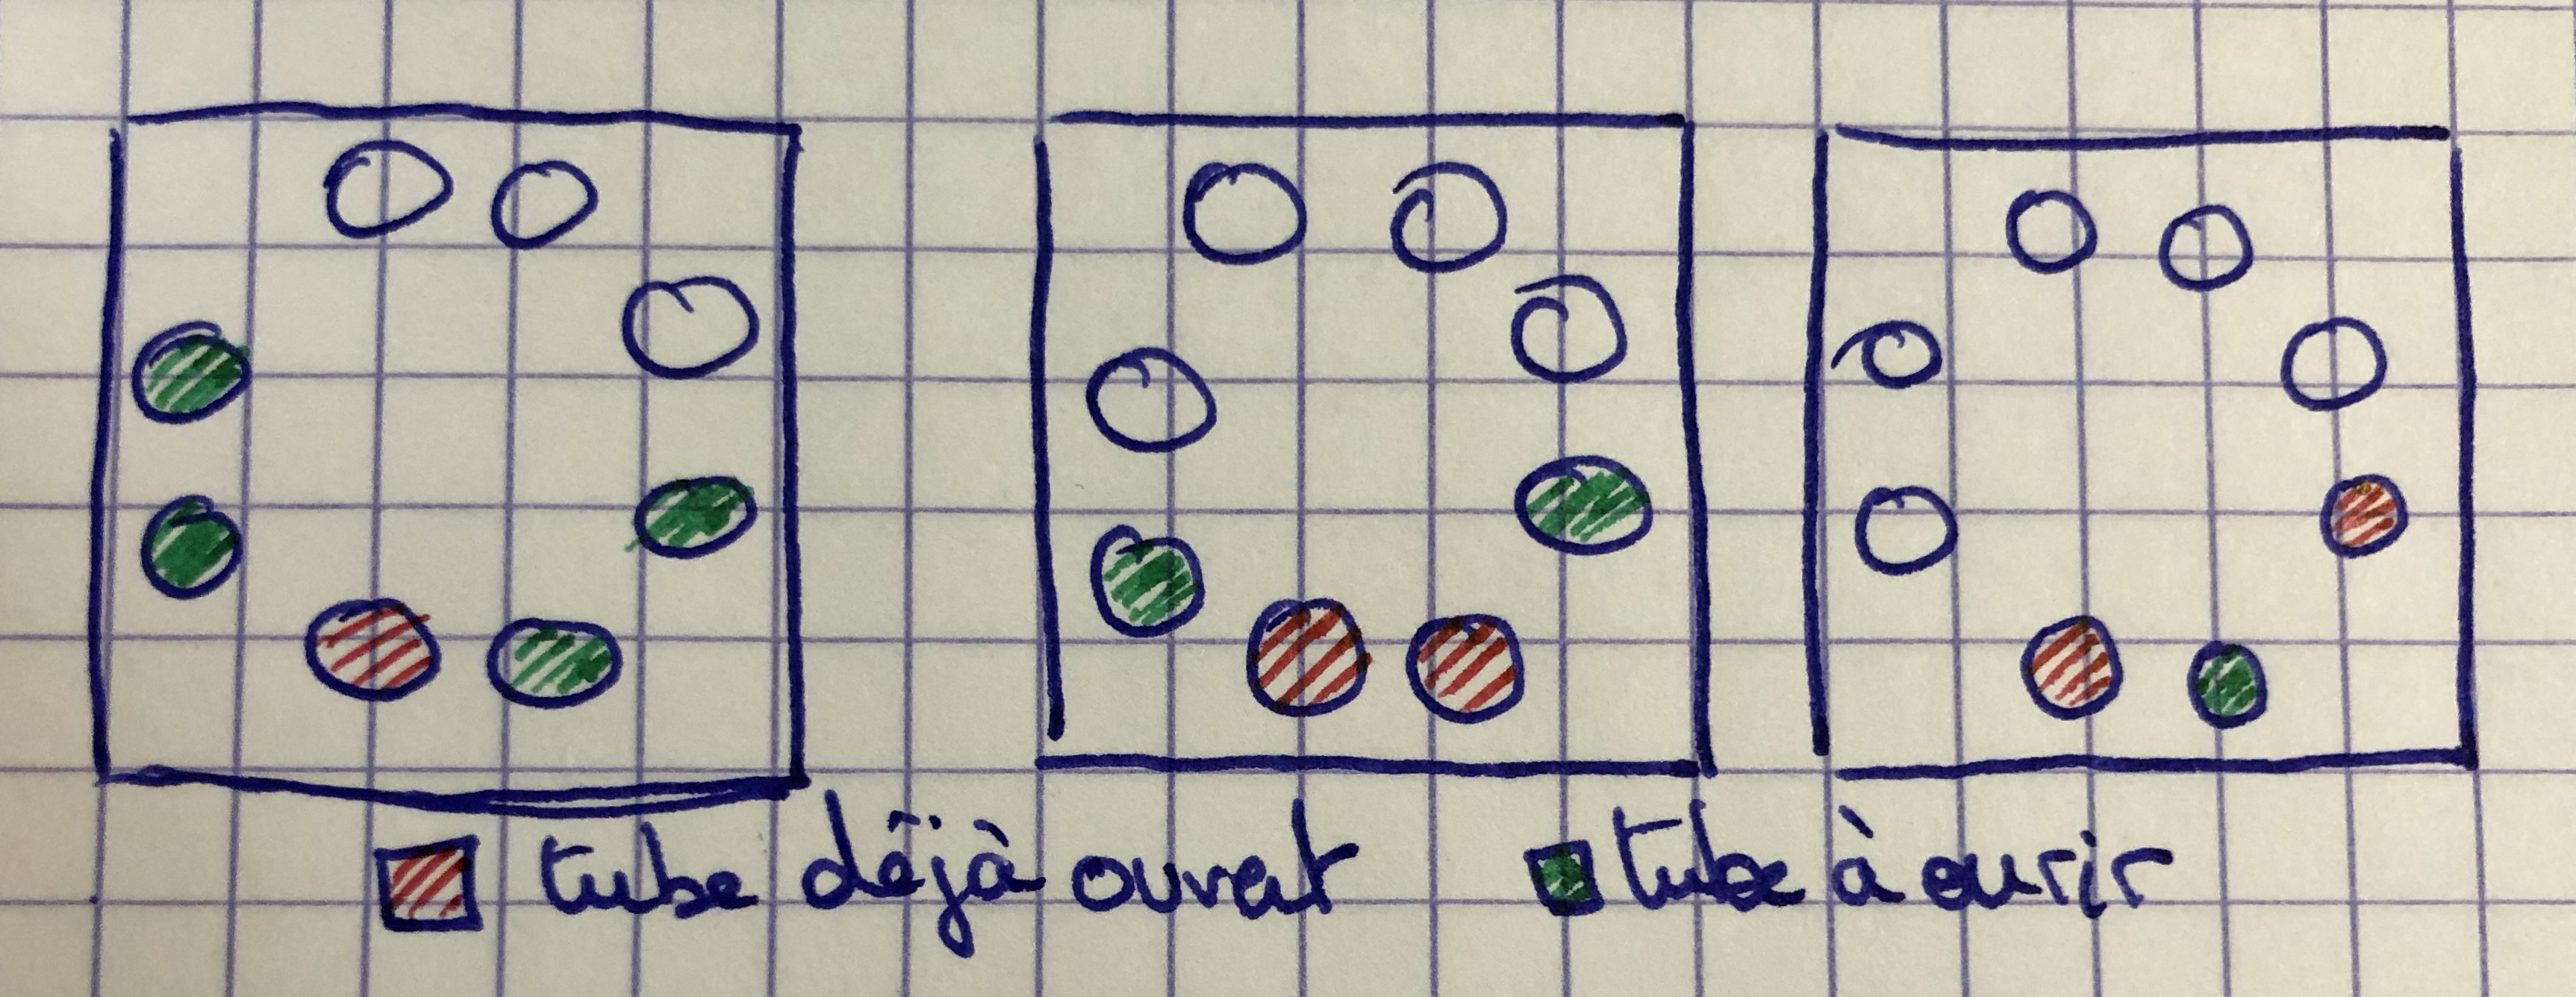
\includegraphics[width=11cm]{PDC-open-tube.jpg}
    \end{center}
    \caption{Tubes à ouvrir selon la situation}
\label{OpenTube}
\end{figure}

\paragraph{}Les tubes du barillier sont numérotés de 0 à 7. Les tubes déjà ouverts sont inclus dans une liste. On suppose que dans la liste, le premier tube est celui le plus à gauche
du groupement de tubes ouverts, le deuxième est le tube ouvert suivant à sa droite, jusqu'au dernier tube qui est le tube ouvert le plus à droite du groupement. C'est à dire que si les
tubes 0, 1 et 7 sont ouverts, la liste sera : \{7,0,1\}. Pour résoudre ce problème, nous avons avons distingué deux situations :
\begin{description}
    \item[Situation 1 :] Tous les tubes ouverts sont accolés
    \item[Situation 2 :] Il y a un ou plusieurs tubes fermés à l'intérieur du groupement de tubes
\end{description}
Dans les deux situations, il faut trouver quels sont les tubes extérieurs au groupement que l'on peut ouvrir. Pour cela, il faut en premier calculer l'étendue du groupement. Tant que
le groupement n'est pas à cheval sur un index 0, tout va bien, on calcule simplement la différence entre l'index du tube le plus à droite et l'index du tube le plus à gauche et on
rajoute 1. Sinon, on doit d'abord ajouter le nombre de tubes du barillier à tous les index qui sont inférieurs à l'index du tube le plus à gauche : si la liste de tube ouverts est
{7,0,1}, elle deviendra {7,8,9}. On peut ensuite appliquer la méthode décrite avant. On applique ensuite une boucle pour trouver les extrémités :
\begin{verbatim}
Pour i allant de l'étendue du groupement au nombre maximum de
tube ouvert :
    min = index tube le plus à gauche
        - (nombre maximum de tubes ouverts - i)
    max = index tube le plus à droite
        + (nombre maximum de tubes ouverts - i)
    Index dans la séquence(min) -> possibilité
    Inde dans la séquence(max) -> possibilité
Fin de la boucle Pour
\end{verbatim}
De cette façon, on obtient toutes les extrémités possibles. Maintenant il faut traiter la seconde situation : si des tubes sont fermés au milieu du groupement de tubes ouverts. Pour
cela, il suffit de parcourir chaque tube à partir du premier jusqu'au dernier du groupement : si le tube est fermé on le rajoute à la liste des possibilités. On obtient donc toutes les
possibilités, il n'y a plus qu'a choisir une possibilité au hasard et ouvrir ce tube.

\paragraph{}Plus haut, j'ai précisé qu'on supposait que la liste des tubes ouverts était triée d'une certaine manière. Apres avoir ouvert le tube, il faut donc ajouter son index au
bon endroit dans la liste des tubes ouverts. Pour cela on doit le comparer avec chaque index de la liste. Cela donne :
\begin{verbatim}
Pour x = chaque index de la liste des tubes ouverts :
    On a i = index du tube a rajouter
    valeur rajoutée = 0
    Si Abs(x - i) > longueur maximum du groupement
        On rajoute + 8 à la plus petite valeur entre x et i
    Si (x > i)
        On intercale l'index du tube à rajouter à
            l'emplacement de x dans la liste
        Stop de la boucle Pour
    Sinon Si x est le dernier élément de la liste
        On place l'index du tube à rajouter à la fin de
            la liste
Fin de la boucle Pour
\end{verbatim}

\newpage
\paragraph{Gestion du score} Concernant le scoring, nous avons décidé de nous inspirer du système de scoring du jeu de rythme Osu. Dans l'image \ref{ScoringInspiration}, on peut voir 4
éléments principaux de scoring. En haut à gauche se trouve une jauge de vie qui baisse à chaque erreur et remonte a chaque rythme réussi. En bas à gauche se trouve le combo de rythmes
réussis d'affilé. Celui-ci est un multiplicateur des points gagnés par rythme réussi. La somme totale des points est affichée en haut à droite, au dessus du pourcentage de réussite sur
la partie. Le scoring sur Osu est détaillé sur leur site internet \cite{OSU}.\\

\begin{figure}[H]
    \begin{center}
    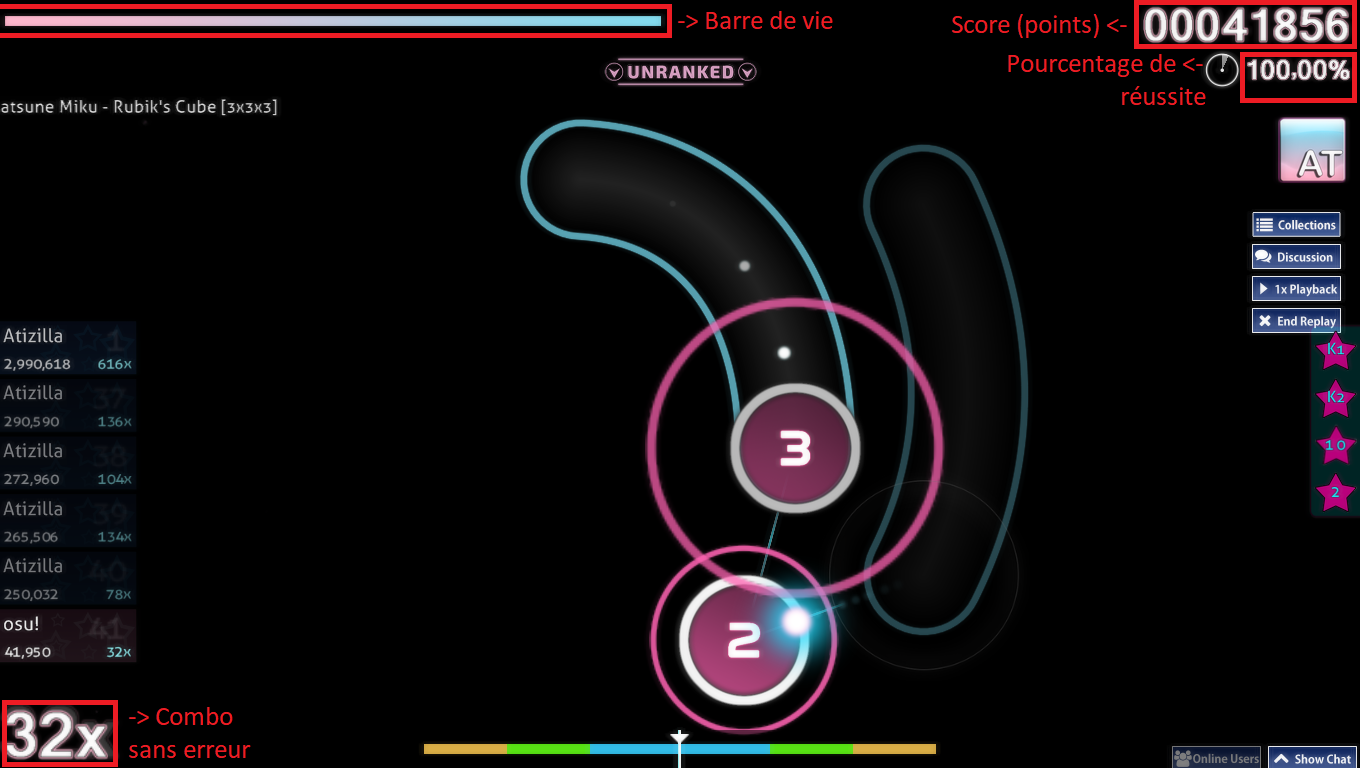
\includegraphics[width=13cm]{osu-scoring-inspiration-description.png}
    \end{center}
    \caption{Le scoring dans Osu}
\label{ScoringInspiration}
\end{figure}

\begin{wrapfigure}[8]{l}{3cm}
    \vspace{-10pt}
    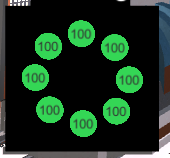
\includegraphics[width=3cm]{PDC-scoring-multi.png}
    \captionsetup{labelformat=simpleNumber}
    \caption{Multi}
\end{wrapfigure}

\paragraph{}Nous avons donc repris ces 4 éléments : il y a soit une jauge de vie qui est commune à tous les tubes, soit une jauge de vie pour chaque tube dans le carré noir en bas à
gauche de l'écran. Si des cibles passent, la jauge de vie baisse de 15. Si celles-ci sont retirées, la jauge remonte de 5. A chaque distracteur qui passe, la barre de vie monte
également de 0.1. Cela permet de faire remonter tout doucement la jauge de vie dans le cas où peu de cibles apparaitraient. Au dessus de la jauge de vie se trouve le combo de réussite
et le score. En bas à droite, la cible est représentée au joueur. La précision de réussite est juste au dessus de la cible.

\begin{figure}[H]
    \begin{center}
    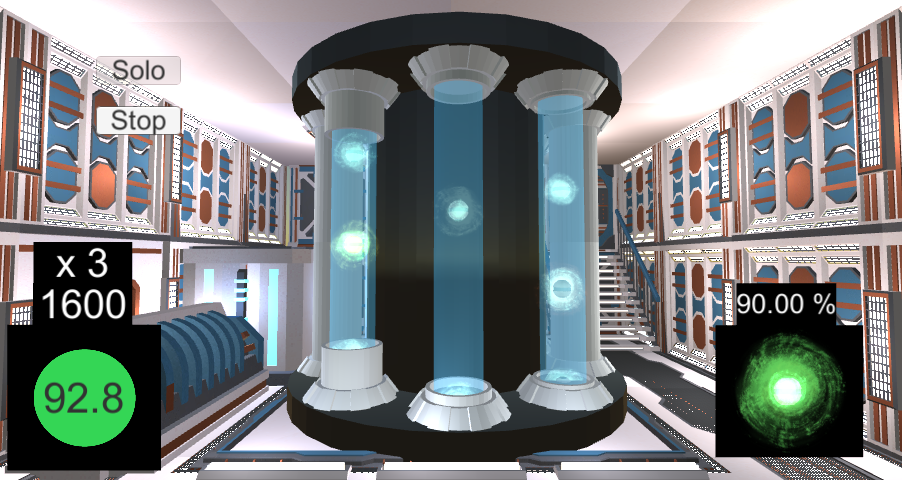
\includegraphics[width=13cm]{PDC-scoring.png}
    \end{center}
    \caption{Le scoring dans notre jeu}
\label{ScoringPDCInspiration}
\end{figure}

\paragraph{}Nous avons quelques perspectives d'amélioration pour ce mini jeu qu'il pourrait être intéressant de développer. Nous avons par exemple pensé à changer la vitesse des
sphères de manière indépendante selon les tubes. Un autre amélioration un peu plus importante du gameplay serait de rajouter des miroirs sur les côtés du barillier pour pouvoir voir
les tubes qui sont cachés derrière et ainsi augmenter le nombre maximum de tubes ouverts.

\label{prototypage}